\documentclass[svgnames,11pt]{beamer}
\setbeamercolor{structure}{fg=SlateGray}
\usetheme{Goettingen}
\input{/home/tof/Documents/Cozy/latex-include/preambule_commun.tex}
\author[]{Christophe Viroulaud}
\title{}
\date{}
%\logo{}
%\institute{Seconde SNT}
%\institute{Première NSI}
\institute{Terminale NSI}
\setbeamertemplate{navigation symbols}{}
\setbeamertemplate{footline}[frame number]
\usepackage{tikz}

\begin{document}
\begin{frame}
\titlepage
\end{frame}
\section{Problématique}

\begin{frame}
    \frametitle{}
    L'approche gloutonne du rendu de monnaie permet de résoudre efficacement un problème mais ne donne pas toujours une solution optimale.
\begin{center}
    \framebox{Peut-on trouver une solution optimale en un temps raisonnable?}
\end{center}

\end{frame}
\section{Approche gloutonne}
\subsection{Algorithme}
\begin{frame}
    \frametitle{L'algorithme glouton fait un choix définitif}
\begin{center}
    \lstinputlisting[firstline=10 ,lastline= 19]{"scripts/rendu-monnaie.py"}
    \captionof{code}{Approche gloutonne}
    \label{glouton}
\end{center}

\end{frame}
\begin{frame}[fragile]
    \frametitle{Exemple d'exécution}

    \begin{center}
        \begin{lstlisting}[language=Python]
systeme = [50, 20, 10, 5, 2, 1]
somme = 8
nb_pieces_glouton(somme, systeme)
        \end{lstlisting}
        \label{moncode}
    \end{center}
    \begin{center}
        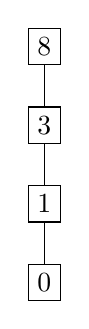
\begin{tikzpicture}
            \node[draw] (A) at (0,0) {8};
            \node[draw] (B) at (0,-1) {3};
            \node[draw] (C) at (0,-2) {1};
            \node[draw] (D) at (0,-3) {0};

            \draw (A) -- (B);
            \draw (C) -- (B);
            \draw (C) -- (D);

        \end{tikzpicture}
        \label{moncode}
    \end{center}
\end{frame}
\subsection{Un exemple non optimal}
\begin{frame}[fragile]
    \frametitle{Un système non optimal (non canonique)}

    \begin{center}
        \begin{lstlisting}[language=Python]
systeme = [30, 24, 12, 6, 3, 1]
        \end{lstlisting}
        \captionof{code}{Système monétaire impérial britannique}
        \label{systeme}
    \end{center}
    \begin{activite}
        Dérouler à la main l'exécution de la fonction \emph{nb\_pieces\_glouton} pour 48€ avec le système (simplifié) de monnaie européenne puis le système impérial.
    \end{activite}
\end{frame}


\begin{frame}
    \frametitle{La solution proposée par l'algorithme glouton}

    \begin{center}
        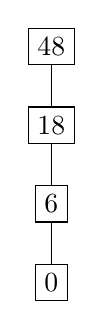
\begin{tikzpicture}
            \node[draw] (A) at (0,0) {48};
            \node[draw] (B) at (0,-1) {18};
            \node[draw] (C) at (0,-2) {6};
            \node[draw] (D) at (0,-3) {0};

            \draw (A) -- (B);
            \draw (C) -- (B);
            \draw (C) -- (D);
        \end{tikzpicture}
        \label{moncode}
    \end{center}

\end{frame}
\begin{frame}
    \frametitle{Une meilleure solution}

    \begin{center}
        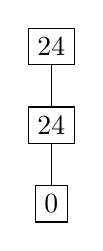
\begin{tikzpicture}
            \node[draw] (A) at (0,0) {24};
            \node[draw] (B) at (0,-1) {24};
            \node[draw] (C) at (0,-2) {0};

            \draw (A) -- (B);
            \draw (C) -- (B);
        \end{tikzpicture}
        \label{moncode}
    \end{center}

\end{frame}
\section{Approche dynamique}
\subsection{Algorithme naïf}
\begin{frame}[fragile]
    \frametitle{Il faut énumérer toutes les possibilités}

    \begin{center}
        \lstinputlisting[firstline=33 ,lastline= 43, basicstyle=\small, xrightmargin=1.8em, xleftmargin=2em]{"scripts/rendu-monnaie.py"}
        \captionof{code}{Approche naïve}
        \label{naif}
    \end{center}

\end{frame}

\begin{frame}
    \frametitle{}

    \begin{center}
        \centering
        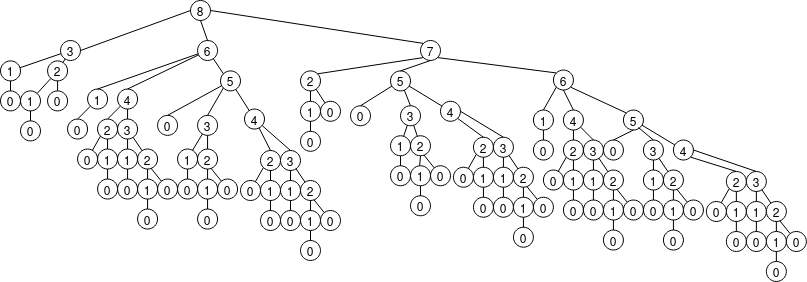
\includegraphics[width=10cm]{ressources/appel-naif-8.png}
        \captionof{figure}{Appels récursifs pour 8€}
        \label{IMG}
    \end{center}
On teste récursivement toutes les solutions pour chaque pièce du système (ligne 6).
\end{frame}

\begin{frame}
    \frametitle{}

    \begin{activite}
        En s'aidant de l'arbre, dérouler l'exécution de la fonction (pour les premiers cas) à la main afin d'en comprendre le fonctionnement.
        \end{activite}

\end{frame}
\begin{frame}
    \frametitle{}

    \begin{itemize}
        \item Choisir 5, reste 3
        \begin{itemize}
            \item Choisir 2, reste 1
            \begin{itemize}
                \item Choisir 1, reste 0 $\;\rightarrow\;$ \\remontée d'appel, nb\_pieces = 1, nb\_mini = 1
            \end{itemize}
            \item Choisir 1, reste 2
            \begin{itemize}
                \item Choisir 2, reste 0
                \item Choisir 1, reste 1\\
                Choisir 1, reste 0 $\;\rightarrow\;$ \\remontée d'appel, nb\_pieces = 1, nb\_mini = 1
                
            \end{itemize}
        \end{itemize}
        \item Choisir 2, reste 6
        \item Choisir 1, reste 7
    \end{itemize}

\end{frame}
\subsection{Top-down}
\begin{frame}
    \frametitle{}

    L'utilisation d'un tableau \emph{track} pour éviter la redondance des calculs.

\end{frame}

\begin{frame}
    \frametitle{}

    \begin{activite}
        \begin{enumerate}
            \item Écrire la fonction \textbf{nb\_pieces\_TD(somme: int, systeme: list, track: list) $\;\rightarrow\;$int} qui reprend l'algorithme naïf et utilise le tableau \emph{track} de stockage intermédiaire.
            \item Tester la fonction pour les deux systèmes monétaires.
        \end{enumerate}
        \end{activite}

\end{frame}

\begin{frame}
    \frametitle{}

    \lstinputlisting[firstline=46 ,lastline= 61, basicstyle=\small, xrightmargin=1.8em, xleftmargin=2em]{"scripts/rendu-monnaie.py"}

\end{frame}
\begin{frame}[fragile]
    \frametitle{}

    \begin{center}
        \begin{lstlisting}[language=Python]
systeme = [10, 5, 2, 1]
somme = 8
# Le tableau de stockage est initialisé
track = [-1 for _ in range(somme+1)]
nb_pieces_TD(somme, systeme, track)
        \end{lstlisting}
        \captionof{code}{Appel de la fonction}
        \label{moncode}
    \end{center}

\end{frame}
\begin{frame}
    \frametitle{Englober le cas limite dans track}

    \lstinputlisting[firstline=64 ,lastline= 74, basicstyle=\small, xrightmargin=1.8em, xleftmargin=2em]{"scripts/rendu-monnaie.py"}

\end{frame}

\begin{frame}[fragile]
    \frametitle{}

    \begin{center}
        \begin{lstlisting}[language=Python]
systeme = [10, 5, 2, 1]
somme = 8
# Le tableau de stockage est initialisé
track = [-1 for _ in range(somme+1)]
track[0] = 0
nb_pieces_TD2(somme, systeme, track)
        \end{lstlisting}
        \captionof{code}{Appel de la fonction}
        \label{moncode}
    \end{center}

\end{frame}

\begin{frame}
    \frametitle{}

    \begin{center}
        \centering
        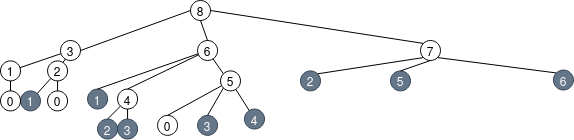
\includegraphics[width=10cm]{ressources/appel-dyn-8.png}
        \captionof{figure}{Approche dynamique pour 8€}
        \label{IMG}
    \end{center}

\end{frame}

\subsection{Bottom-up}
\begin{frame}[fragile]
    \frametitle{Approche itérative}

    \begin{center}
        \lstinputlisting[firstline=77 ,lastline= 88, basicstyle=\small]{"scripts/rendu-monnaie.py"}
        \captionof{code}{Approche bottom-up}
        \label{bu}
    \end{center}

\end{frame}
\begin{frame}[fragile]
    \frametitle{Le tableau se remplit d'abord par les petites valeurs}

    \begin{itemize}
        \item<1-> \begin{lstlisting}[language=Python]
track = [0, 0, 0, 0, 0, 0, 0, 0]
        \end{lstlisting}
        \item<2-> \begin{lstlisting}[language=Python]
track = [0, 1, 0, 0, 0, 0, 0, 0]
        \end{lstlisting}
        \item<3-> \begin{lstlisting}[language=Python]
track = [0, 1, 1, 0, 0, 0, 0, 0]
        \end{lstlisting}
        \item<4-> \begin{lstlisting}[language=Python]
track = [0, 1, 1, 2, 0, 0, 0, 0]
        \end{lstlisting}
        \item<5-> \begin{lstlisting}[language=Python]
track = [0, 1, 1, 2, 2, 0, 0, 0]
        \end{lstlisting}
    \end{itemize}

\end{frame}
\begin{frame}
    \frametitle{}

    \begin{activite}
        Écrire la fonction \textbf{nb\_pieces\_BU\_sol(somme: int, systeme: list) $\;\rightarrow\;$ list} qui renvoie la liste des pièces à choisir pour rendre la monnaie. On utilisera un tableau \emph{choix} de taille \emph{somme+1} où chaque élément de rang x contiendra la valeur de la première pièce à rendre pour la somme x.
        \end{activite}

\end{frame}
\begin{frame}
    \frametitle{Création des stockages}

    \lstinputlisting[firstline=91 ,lastline= 94, basicstyle=\small, xrightmargin=2em, xleftmargin=2em]{"scripts/rendu-monnaie.py"}
\begin{aretenir}[Remarque]
On aurait également pu utiliser un dictionnaire pour stocker les choix de pièces effectués: la clé est la somme à rendre et la valeur correspondante la première pièce à rendre.
\end{aretenir}
\end{frame}
\begin{frame}
    \frametitle{Remplissage des stockages}

    \lstinputlisting[firstline=95 ,lastline= 105, basicstyle=\small, xrightmargin=2em, xleftmargin=2em]{"scripts/rendu-monnaie.py"}

\end{frame}
\begin{frame}
    \frametitle{Reconstruction de la solution}

    \lstinputlisting[firstline=106 ,lastline= 112, basicstyle=\small, xrightmargin=2em, xleftmargin=2em]{"scripts/rendu-monnaie.py"}

\end{frame}
\end{document}